\documentclass[
portrait,
%landscape,
a0paper%,
%draft
]
{baposter}
%
% load packages
% already loaded some useful packages for figures, tables and layout
% not all are needed to run this minimal example
\usepackage{graphicx}
\usepackage[percent]{overpic}
\usepackage[detect-weight]{siunitx}
\usepackage{tabto}
\usepackage{booktabs}
\usepackage{amsmath}
\usepackage{float}
\usepackage{multirow}
\usepackage{multicol}
\usepackage{url}
\usepackage{enumitem}
\usepackage{tikz}
\usepackage{pgfplots}
\usepackage{colortbl}
\usepackage{makecell}
\usepackage{caption}
\usepackage{subcaption}
\usepackage{varwidth}
\pgfplotsset{compat=1.18}
% add additional packages you need here
%
% for now usig bibitem, but if you want ...
%\usepackage[backend=biber]{biblatex} 
%
% customizing 
\newlength{\mytextsize}
\newcommand\e{\cdot 10^}
\setlength{\unitlength}{1.0cm}
%
% define colors
\definecolor{unswyellow}{cmyk}{0,0.05,1,0} %for text / color / logo
\definecolor{unswRed1}{cmyk}{0, 1, 1, 0}
\definecolor{unswRed2}{cmyk}{0, 1, 1, 0.2}
\definecolor{unswRed3}{cmyk}{0, 1, 1, 0.4}
\definecolor{unswRed4}{cmyk}{0, 1, 1, 0.6}

% fonts
\usepackage[scaled]{helvet}
\renewcommand*\familydefault{\sfdefault}

% TikZ banner
\newcommand{\unswBanner}{
    
\begin{tikzpicture}
    % Segment 1
    \fill[unswRed1] (-0.1,0) -- (6.8,0) -- (7,0.4) -- (6.8,0.8) -- (-0.1,0.8) -- cycle;
    \node[white, font=\bfseries, align=center] at (1.35,0.4) {\normalsize Australia's Global University};

    % Segment 2 (with arrow shape)
    \fill[unswRed2] (6.8,0) -- (11.4,0) -- (11.6,0.4) -- (11.4,0.8) -- (6.8,0.8) -- (7,0.4) -- cycle;
    \node[white, font=\bfseries, align=center] at (7.5,0.4) {\normalsize Faculty of Engineering};

    % Segment 3 (with arrow shape)
    \fill[unswRed3] (11.4,0) -- (21.6,0) -- (21.8,0.4) -- (21.6,0.8) -- (11.4,0.8) -- (11.6,0.4) -- cycle;
    \node[white, font=\bfseries, align=center] at (12,0.4) {\normalsize School of Electrical Engineering and Telecommunications};

    \fill[unswRed4] (21.6,0) -- (26,0) -- (26,0.8) -- (21.6,0.8) -- (21.8, 0.4) -- cycle;
  \end{tikzpicture}
}

%
%
%##################################################################################
\begin{document}
%##################################################################################
\begin{poster}
{
  % options
  grid=false,
  background=plain,
  bgColorOne=white,
  columns=6,
  eyecatcher=false,
  borderColor=unswyellow,
  headerColorOne=unswyellow, %white,
  headershade=plain,
  %headerColorTwo=white,
  headerborder=open,
  % for rectangular boxes change the next two options, rectangular header will cause left aligning of box title 
  textborder=rounded, %rectangle,
  headershape=rounded, %rectangle,
  headerfont=\bf\large,
  boxshade=none,
  headerFontColor=black, %white,
  headerheight=0.14\textheight
}
{
  %eyecatcher ...
}
{
%   %poster title
%   % first put graphics for header
  \begin{picture}(23.7, 2.1)
  \fboxsep
  \put(-0.6, -2){\colorbox{unswyellow}{\rule[190pt]{800pt}{0pt}}}
  \thicklines
  % minipage box for title and authors
  \put(2.55, 1.7){
    \begin{minipage}[t][96pt]{0.9\textwidth}
    % centering
    \begin{center}
    % Title
    % use \LARGE instead of \Huge for long titles, you might need to modify distances or number of lines
    % for one line title
    \ \vspace{0.15cm}\\
    \huge\bf\color{black}\selectfont Single Line Title \vspace{0.4cm}\\ 
    % for two line title
    % \Huge\bf\color{black}\selectfont Two Line Title 
    % \vspace{0.1cm} \\ 

    % \vspace{0.2cm}
    \textmd{
    \huge\textit{Author:} \\ 
    \vspace{-0.5em}
    \Large\textit{Supervisor:}} \\
    \end{center} 
  \end{minipage}}
  \put(1,-1.2){\includegraphics[height=75pt]{Figure/UNSW_logo.png}}
  \end{picture} 
}
{
    \put(-0.7, -2){\unswBanner}
}
{
	%logo, already in title
}

\headerbox{Introduction}{name=intro, span=3, row=0, column=0}{
\begin{itemize}[noitemsep,topsep=0pt,parsep=0pt,partopsep=0pt, leftmargin=10pt]
    \item Point 1
    \item Point 2
    \item Point 3
\end{itemize}
}

\headerbox{My Research Methodology}{name=meth, span=6, below=intro, column=0}{
    \begin{multicols}{2}
    \begin{figure}[H]
        \centering
        \includegraphics[width=0.45\textwidth]{Figure/Figure1.pdf}
        \captionsetup{margin={.4em,0.4em}}
        \caption{Method 1}
    \end{figure}
    \begin{figure}[H]
        \centering
        \includegraphics[width=0.45\textwidth]{Figure/Figure2.pdf}
        \captionsetup{margin={.4em,0.4em}}
        \caption{Method 2}
    \end{figure}
    \end{multicols}
}

\headerbox{Key Challenges}{name=challenge, span=3, row=0, column=3, above=meth}{
\begin{itemize}[noitemsep,topsep=0pt,parsep=0pt,partopsep=0pt, leftmargin=10pt]
    \item Challenge 1
    \item Challenge 2
    \item Challenge 3
\end{itemize}
}

\headerbox{My Thesis Outcome}{name=workload, span=2, column=0, below=meth, above=bottom}{
\begin{center}
\vspace{0.5em}
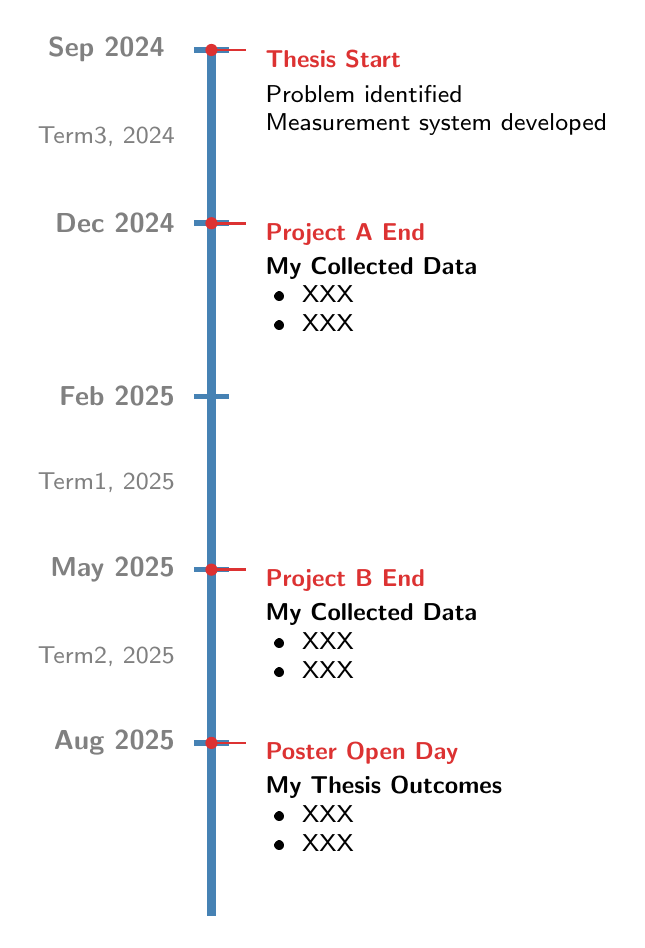
\begin{tikzpicture}[scale=1.1,transform shape]
% Define colors
\definecolor{timelineblue}{RGB}{70,130,180}
\definecolor{eventred}{RGB}{220,50,50}

% Timeline parameters
\def\timelinestart{0}
\def\timelineend{10}
\def\timelinewidth{1}

% Draw main vertical timeline (top to bottom)
\draw[line width=3pt,timelineblue](0,\timelineend)--(0,\timelinestart);

% Month labels and markers (top to bottom)
\pgfmathsetmacro{\sep}{0}
\pgfmathsetmacro{\dec}{2}
\pgfmathsetmacro{\feb}{4}
\pgfmathsetmacro{\may}{6}
\pgfmathsetmacro{\aug}{8}
\foreach \i/\month in {
\aug/Aug 2025,
\may/May 2025,
\feb/Feb 2025,
\dec/Dec 2024,
\sep/Sep 2024
}{
  \pgfmathsetmacro{\y}{\timelineend - \i}
  \draw[line width=2pt,timelineblue](-0.2,\y)--(0.2,\y);
  \node[left,align=right,font=\small\bfseries] at (-0.3,\y) {\textcolor{gray}{\month}};
}

% Terms (adjusted for top-down direction)
    % \node[above, align=center, font=\footnotesize] at (3*1.5/2, 0.5) {\textcolor{gray}{Term 3, 2024}};

\node[left,font=\footnotesize,align=right] at (-0.3,{\timelineend - \dec/2}) {\textcolor{gray}{Term3, 2024}};

\node[left,font=\footnotesize,align=right] at (-0.3,{\timelineend - (\feb + (\may - \feb)/2)}) {\textcolor{gray}{Term1, 2025}};

\node[left,font=\footnotesize,align=right] at (-0.3,{\timelineend - (\may + (\aug - \may)/2)}) {\textcolor{gray}{Term2, 2025}};

% Events
% ThesisStart
\pgfmathsetmacro{\y}{\timelineend - \sep}
\node[anchor=north west,yshift=0.35em,align=left,font=\footnotesize] at (0.5,\y) {
  \textcolor{eventred}{\textbf{Thesis Start}}\\[2pt]
  \textcolor{black}{Problem identified}\\
  \textcolor{black}{Measurement system developed}
  
};
\draw[eventred, line width=1pt](0,\y)--(0.4,\y);
\fill[eventred](0,\y) circle(2pt);

% ProjectAEnd
\pgfmathsetmacro{\y}{\timelineend - \dec}
\node[anchor=north west,yshift=0.35em,align=left,font=\footnotesize] at (0.5,\y) {
  \textcolor{eventred}{\textbf{Project A End}}\\[3pt]
  \begin{varwidth}{8cm}
    \textbf{My Collected Data}
    \begin{itemize}[noitemsep,topsep=0pt,leftmargin=12pt]
      \item XXX 
      \item XXX
    \end{itemize}
  \end{varwidth}
};
\draw[eventred, line width=1pt](0,\y)--(0.4,\y);
\fill[eventred](0,\y) circle(2pt);

% ProjectBEnd
\pgfmathsetmacro{\y}{\timelineend - \may}
\node[anchor=north west,yshift=0.35em,align=left,font=\footnotesize] at (0.5,\y) {
  \textcolor{eventred}{\textbf{Project B End}}\\[3pt]
  \begin{varwidth}{8cm}
    \textbf{My Collected Data}
    \begin{itemize}[noitemsep,topsep=0pt,leftmargin=12pt]
      \item XXX 
      \item XXX
    \end{itemize}
  \end{varwidth}
};
\draw[eventred, line width=1pt](0,\y)--(0.4,\y);
\fill[eventred](0,\y) circle(2pt);

% PosterOpenDay
\pgfmathsetmacro{\y}{\timelineend - \aug}
\node[anchor=north west,yshift=0.35em,align=left,font=\footnotesize] at (0.5,\y) {
  \textcolor{eventred}{\textbf{Poster Open Day}}\\[3pt]
  \begin{varwidth}{4.3cm}
    \textbf{My Thesis Outcomes}
    \begin{itemize}[noitemsep,topsep=0pt,leftmargin=12pt]
      \item XXX 
      \item XXX
    \end{itemize}
  \end{varwidth}
};
\draw[eventred, line width=1pt](0,\y)--(0.4,\y);
\fill[eventred](0,\y) circle(2pt);
\end{tikzpicture}

  
\end{center}
% \vspace{-3em}

}

\headerbox{My Analysis Results}{name=results, span=4, column=2, below=meth, above=bottom}{
\begin{figure}[H]
    \centering
    \includegraphics[width=0.35\textwidth]{Figure/Results_1.pdf}
    \vspace{-0.5em}
    \captionsetup{margin={.4em,0.4em}}
    \caption{Results 1}
\end{figure}
\vspace{-1em}
\begin{figure}[H]
    \centering
    \begin{subfigure}{0.35\textwidth}
    \includegraphics[width=\linewidth]{Figure/Results_2.pdf}
    \caption{Results 2}
    \end{subfigure}
    \hspace{2em}
    \begin{subfigure}{0.35\textwidth}
    \includegraphics[width=\linewidth]{Figure/Results_3.pdf}
    \caption{Results 3}
    \end{subfigure}
\end{figure}
}

\end{poster}
\end{document}
